\documentclass{beamer}
\usepackage{graphicx}
\graphicspath{ {./images/} }

\title{WaterWizards}
\author{Justin Dewitz, Max Kondratov, Erick Zeiler, Julian <Nachname>}
\date{17. Juli 2025}

\begin{document}

\frame{\titlepage}

\begin{frame}
\frametitle{Inhaltsverzeichnis}
\tableofcontents
\end{frame}

\section{Demo + Einleitung}
\begin{frame}
\frametitle{Demo + Einleitung}
\begin{itemize}
  \item Was ist WaterWizards?
  \begin{enumerate}
    \item Mulitplayer Real-Time Schiffe versenken
    \item Angriff durch Zauber, die durch Karten repräsentiert werden
    \item Ziel: Zerstörung der gegnerischen Schiffe
  \end{enumerate}
  \item Warum WaterWizards?
  \begin{enumerate}
    \item Schiffe versenken ist ein Klassiker
    \item Durch Real-Time wird es dynamischer
    \item Für jede Altersgruppe interessant
  \end{enumerate}
\end{itemize}
\end{frame}

\section{Organisation}
\begin{frame}
  \frametitle{Organisation}
  \begin{itemize}
    \item git über GitHub für die Versionsverwaltung 
    \item Scrum mit 2-Wochen-Sprints
    \item Kanban/Issue-Board über GitHub
    \item Kommunikation über Discord-Server
  \end{itemize}
\end{frame}

\section{Rollen des Projektes}
\begin{frame}
\frametitle{Rollen des Projektes}

\end{frame}

\subsection{Ansprechpartner}
\begin{frame}
\frametitle{Ansprechpartner}

\end{frame}

\section{Technologie + Architektur}
\begin{frame}
\frametitle{Backend - Client Kommunikation}
\begin{columns}
  \begin{column}{0.55\textwidth}
    \begin{itemize}
      \item LiteNetLib für die Client-Server-Verbindung
      \begin{enumerate}
        \item UDP für die Echtzeit-Kommunikation
        \item Nachrichten basiertes Protokoll für beidseitige Kommunikation
      \end{enumerate}
      \item Event-Driven Architektur
    \end{itemize}
  \end{column}
  \begin{column}{0.7\textwidth}
    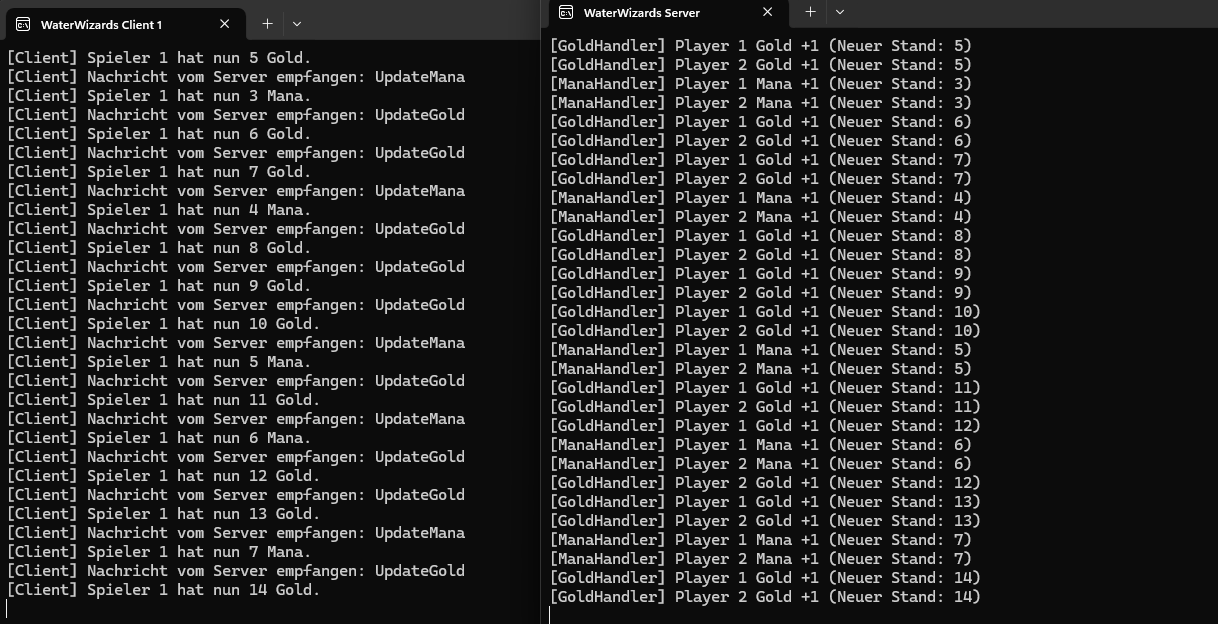
\includegraphics[width=\textwidth]{Server-Client-Logs.png}
  \end{column}
\end{columns}
\end{frame}

\subsection{UI}
\begin{frame}
  \frametitle{UI}
\end{frame}

\subsection{GameScreen}
\begin{frame}
\frametitle{GameScreen}
  GameScreen enthält alles, was auf dem Bildschirm gezeigt wird:
  \begin{enumerate}
    \item Die beiden Spielbretter (GameBoard) mit Schiffen (GameShip) und Steinen
    \item Die Karten (GameCard) auf der Hand (GameHand) der Spieler
    \item Die Kartenstapel (CardStack) der einzelnen Kartentypen (CardType)
  \end{enumerate}
\end{frame}


\subsection{Server/Backend}
\begin{frame}
\frametitle{Server/Backend}
\end{frame}

\subsection{Shared}
\begin{frame}
\frametitle{Shared}
\end{frame}

\subsection{Backend - Client Kommunukation}
\begin{frame}
\frametitle{Backend - Client Kommunikation}
\end{frame}

\section{Wiki}
\begin{frame}
\frametitle{Wiki}

\end{frame}

\section{Erfahrungen und Fazit}
\begin{frame}
\frametitle{Erfahrungen und Fazit}

\end{frame}

\end{document}